
\section{Comparing Returns and Distribution measures}\label{return_section}
The biggest difference do not appear when using different kinds of weights ("dollar" or "share" method) but rather when building the portfolio from prices or returns. 
Moreover, Fedyk and Welch build their portfolio only using common american stocks (share code 10 or 11). 
In my final analysis I look at all types of securities but significant differences emerge even when using the same sample. 
Additionally, by recreating their method employed by the other authors we can analyse its return when dealing with all kinds of securities. 
In section \ref{diff_samples} I compare returns using only common stocks or the full sample of securities, in the other sections of this paper I will use the full sample unless explicitly stated.

As the other authors have claimed in their papers, the Portfolio built directly from returns had a significantly higher cumulative return compared to the market and positive alpha.

I will proceed to analyse in more detail the distribution of returns of different Robinhood portfolios, showing that my method depicts a far less rosy picture of the "Robinhood strategy".

Moreover, \cite{Fedyk2024} has analysed extensively the differences between the portfolio obtained using the share method and the dollar method. 
We'll focus on the dollar method since it is the same approach I use to compute weights.

\subsection{Constructing Moving Averages}
I begin by computing daily log returns as $r = \ln\left(\frac{P_1}{P_0}\right)$, knowing that for small $x$, $\ln(1+x)\approx x$. 
Defining log returns allows us to simply compute moving averages, showing the profitability of the Robinhood portfolio at different time frames.
Conceptually, the value of an $n$-day moving average on a given date $T$ represents the return an investor would have earned by initiating the position at the open of day $T-n$ and holding it continuously up to close of day $T$.
More rigorously, for a given horizon of $n$ days:
\begin{equation}
    r_n = \sum_{t=T-n+1}^{T} r_t \approx \ln \left( \prod_{t=T-n+1}^{T} (1+R_t) \right)
\end{equation}
where $r_t$ are dauly log returns and $R_t$ are daily percentage returns.


\subsection{Retail Performance Under Different Samples}\label{diff_samples}




\subsubsection{Rolling Returns Across Investment Horizons}
\paragraph{Common Stocks Only}\label{fedyk_paper_returns}
At short horizons (5–30 days), the two Robinhood portfolios (Fedyk and Mine) display highly similar dynamics, with both closely tracking market indices and exhibiting bursts of volatility during periods of market stress, particularly around the onset of the COVID-19 crash. 
This suggests that in the very short term, retail investors tend to move in tandem with broader market trends, with limited divergence in return profiles across methodologies.
However, at the 120-day horizon, both Robinhood portfolios outperform the S\&P 500 and a World ETF\footnote{I've used Vanguard's VOO for the S\&P500 and Vanguard's VT as a World Equity ETF}. 

This finding is consistent with the idea that many retail investors, especially on Robinhood, engaged in "buy-the-dip" behavior during the COVID-19 crash. 
Their increased exposure to beaten-down or speculative stocks during the downturn appears to have been rewarded in the subsequent rebound. 
Importantly, this also coincides with a period of explosive growth for the platform itself, which may have amplified attention and capital inflows into popular names.

Nonetheless, this post-crash outperformance comes after a prolonged period of clear underperformance. 
Prior to March 2020, both Robinhood portfolios consistently lag behind the benchmark indices, with my method in particular reflecting substantial drawdowns and poor stock selection.

What differentiates the two methods most clearly is the strength of the post-COVID recovery. 
While Fedyk’s method shows a relatively steady climb, my price-based approach rebounds even more sharply after March 2020. 
This reflects the fact that, under my methodology, investor positions are not rebalanced away from prior favorites. 
As a result, stocks that surged after the crash contributed disproportionately to the portfolio’s recovery. 

In sum, the 120-day results provide two key insights: first, that retail traders on Robinhood did benefit from post-crisis market dynamics, and second, that the magnitude and nature of this benefit depends heavily on the modeling approach, particularly when capturing persistence in portfolio composition.

\begin{figure}[h!]
    \centering
    \includegraphics[width=1\linewidth]
    {../images/returns/comparison_1.png}
    \caption{Rolling log-returns of Robinhood and market portfolios at four investment horizons (stock-only sample)}
\end{figure}

\paragraph{Full Universe of Securities}

We now extend the analysis to all securities in the dataset, including ETFs, REITs, and structured products.

Expanding the sample, we still observe that short-term movements (5–30 days) remain closely correlated across all portfolios, with limited divergence in returns or volatility between methods.

However, the performance gap widens at longer horizons. 
In contrast to the stock-only case, where both Robinhood portfolios outperform after the crash, here the drawdowns, particularly in the price-based portfolio, are deeper and more persistent.

Low performance spans the entire pre-COVID period: my portfolio underperforms continuously throughout 2019, while Fedyk’s stays closer to the benchmarks but still lags in absolute terms.

At the 563-day horizon, both Robinhood portfolios end below the S\&P 500 and the World ETF.
My portfolio, while showing a stronger post-crash rebound, barely catches up to the S\&P 500 by the end of the sample, and only due to its heavier exposure to post-crash winners.
Fedyk’s method performs slightly better but remains clearly below the benchmark, reversing the apparent outperformance seen in the stock-only sample.

\begin{figure}[h!]
    \centering
    \includegraphics[width=1\linewidth]
    {../images/returns/comparison_2.png}
    \caption{Rolling log-returns of Robinhood and market portfolios at four investment horizons (complete sample)}
\end{figure}

A detailed description of the distributions can be found in table \ref{tab:returns_all}.

\subsubsection{Distribuional insights}
\paragraph{Common Stocks Only}

The distribution of returns across horizons provides further evidence on the differences between the Robinhood portfolios and the benchmarks.

At short horizons (5–30 days), all portfolios are tightly centered around zero, with relatively similar dispersion. 
Both Robinhood portfolios display slightly higher volatility than the S\&P 500 and the World ETF, with standard deviations of approximately 0.045 for five-day returns, compared to about 0.03 for the benchmarks. 
However, mean returns remain close to zero for all portfolios, and short-term behavior shows limited divergence across methods.

At the 120-day horizon, differences become more evident. 
While Fedyk's portfolio maintains a positive mean log return of approximately 0.05, my price-based portfolio exhibits a negative mean return of about -0.06. 
The median is also much worse, at about -0.14 versus -0.02.
This shift is reflected in the distribution shapes, with my portfolio showing a wider left tail and greater dispersion relative to both Fedyk’s method and the benchmarks.

At the 563-day horizon, the gap further widens. 
The price-based portfolio remains centered around negative returns, with a mean log return of approximately -0.04, while the rebalanced portfolio achieves a positive mean return of 0.17. 
In contrast, the S\&P 500 maintains a strong positive outcome, with a mean log return close to 0.1. 

Despite the strong rebound observed after the COVID-19 crash, the cumulative performance of the price-based portfolio remains significantly weaker, often with higher standard deviation.

\begin{figure}[h!]
    \centering
    \includegraphics[width=1\linewidth]
    {../images/distributions/comparison_1.png}
    \caption{Distribution of rolling log-returns for retail and benchmark portfolios across investment horizons (stock-only sample)}
\end{figure}


A detailed description of the distributions can be found in table \ref{tab:returns_stocks}.

\paragraph{Full Universe of Securities}

Expanding the analysis to include all types of securities slightly alters the distributional patterns compared to the stock-only case.

At short horizons (5–30 days), return distributions remain centered around zero and maintain a similar dispersion across all portfolios. 
Standard deviations are comparable to the stock-only case, around 0.02 for both Robinhood portfolios at the daily level and 0.04 for five-day returns. 
Mean returns are very close to zero, confirming that short-term dynamics are largely unaffected by the broader sample.

At the 120-day horizon, however, differences become more evident. 
Both Robinhood portfolios exhibit flatter distributions with thicker left tails compared to the benchmarks. 
In particular, my price-based portfolio records a negative mean log return of approximately -0.07, while Fedyk’s method also turns slightly negative at around -0.004, unlike in the stock-only case where it remained positive. 
The S\&P 500 maintains a positive mean return over the same horizon, reinforcing the relative weakness of retail portfolios when more asset types are included.

At the cumulative horizon, the gap becomes substantial. My portfolio shows a strongly left-skewed distribution with a mean log return of approximately -0.10.
Fedyk’s portfolio, although positive at around 0.087, remains below the S\&P 500, which achieves a mean return close to 0.1. 
The World ETF again displays lower returns, in line with its broader exposure to international markets.
\begin{figure}[h!]
    \centering
    \includegraphics[width=1\linewidth]
    {../images/distributions/comparison_2.png}
    \caption{Distribution of rolling log-returns for retail and benchmark portfolios across investment horizons (complete sample)}
\end{figure}

Descriptive statistics supporting these findings are reported in Table \ref{tab:returns_all}.

\subsection{Analysis of Short-Term Returns and the Impact of COVID}
Comparing the daily returns for the whole period available we can already observe distinct behavior in terms of returns and distributions for the market and Robinhood indeces.
To test whether there are statistically significant differences beteen the mean daily returns of the Robinhood portfolios, the S\&P 500 and the world ETF, I conduct an ANOVA test.
The null hypothesis is that all portfolios have equal mean daily returns.

\subsubsection{Covering the Whole Period}
As expected from the results regarding the cumulative returns, mean daily returns are very similar for the Robinhood Portfolios.
Fedyk's method has a mean of 0.000555, while the method based on prices has a mean of 0.000450.
The ANOVA analysis conducted on these two portfolios, equal to a t-test in this case, has a p-value of 0.9273.
This suggests that at the daily frequency the expected growth rate, i.e. the mean log returns, of the Robinhood portfolios are not statistically different.


In terms of standard deviation, the Robinhood portfolios have relatively larger values, around 0.02, while the market indeces hvae values around 0.15. 
This is consistent with what can be seen from the distributions: retail portfolios have fatter tails while modal returns appear similar across all timeseries.

Conducting ANOVA tests on all possible combinations of these four timeseries, none has an acceptable p-value, results are in table \ref{tab:anova_all}.
However, conducting a Fligner test to assess difference in variances, the Robinhood portfolios show statistically significant differet variances than the market proxies, results are in table \ref{tab:fligner_all}.


Here below the plots of the distributions, while the returns are in table \ref{tab:returns_all}:
\begin{figure}[h!]
    \centering
    
\includegraphics[width=1\linewidth]
    {../images/distributions/st_all.png}
    \caption{Distribution of daily log-returns for retail and benchmark portfolios (complete sample)}
\end{figure}


\subsubsection{Excluding COVID}
This results on daily returns, however, are probably impacted by the noise of the March 2020 crash. 
I run the same analysis filtering the dataframe up to February 3rd 2020, the date in which the pandemic was declared in the US.

In this case point estimates for means differ greatly even among Robinhood Portfolios, with the price based approach yielding -0.000328 on average versus Fedyk's 0.000246.
Nonetheless, also at this level returns are not statistically significant, results can be found in table \ref{tab:anova_before}.

In terms of standard deviation, the market indices show again clearly a different distribution, with variances being markably lower. 
This is corroborated by fligner tests, available in table \ref{tab:fligner_before}.

Here below the plots of the distributions, while the returns are in table \ref{tab:returns_st_before}:
\begin{figure}[H]
    \centering
    
\includegraphics[width=1\linewidth]
    {../images/distributions/st_before.png}
    \caption{Distribution of daily log-returns for retail and benchmark portfolios (complete sample, excluding COVID)}
\end{figure}

\subsection{Comments}
Daily returns show a deceptively optimistic view, with the different series having statistically equal log-returns.
However, the retail portfolios carry systematically higher day-to-day risk, amd this compounds as underperformance at the cumulative level before the pandemic.

A one-way ANOVA on daily log returns fails to reject equality of means for any group of series, both including and excluding the pandemic. 

However, looking at the risk dimension, stand deviations differ sharply. 
Fligner-Killeen tests reject homogeneity at any $\alpha$ level whenever a retail series is compared with a market proxy.
As highlighted earlier, this can be easily seen from the shape of the distributions, with correspondingly fatter tails.
In log space, larger dispersion automatically lowers long-run growth because every large swing pulls the cumulative sum away from the average trend.
In other words, retail investors accept more noise than the market but earn no meaurable extra drift in a single day.

Although ANOVA cannot reject equality between the Robinhood portfolios, the point estimates themselves are not identical (compare table \ref{tab:returns_st_before}).
The gap in their mean returns, about -0.0006 log points, rapidly cumulates to -0.25 log points. 
The test lacks power because daily $\sigma$ is large; the economic impact measured in compounding is evident.

Path dependence widens the difference.
The price-weighted series \ref{returns_mine} embeds a negative correlation between returns and remaining capital.
When a stock falls, its contribution to the portfolio value shrinks, and therefore any subsequent rebound is applied to less capital, exactly how a normal portfolio would work. 
The return-weighted construction re-anchors weights every market close and therefore avoids this drag.
Losses in early 2019 thus penalise the price-weighted portfolio twice.  





%% -------------------------------------------------------------------- %%
%\subsubsection{old}
%
%We can start by loo
%
%
%
%At short-term horizons (5 to 15 days), all three portfolios show similar patterns, with relatively mild fluctuations. Retail returns exhibit slightly higher volatility, particularly for the Robinhood portfolio, indicating that retail investors are more reactive to short-term market movements. The returns across these horizons reflect a degree of correlation, suggesting that, over short periods, retail investors' behavior mirrors that of the broader market, albeit with more pronounced movements.
%
%At the 30- and 60-day horizons, divergence becomes more apparent. The Robinhood portfolio shows a higher degree of volatility, with both larger peaks and deeper troughs compared to the market and the ETF benchmarks (VOO and VT). This volatility suggests that retail traders may be engaging in more speculative behavior or reacting strongly to market news, which could lead to exaggerated responses and momentum chasing. Notably, during periods of rapid market movements (e.g., mid-2020), the Robinhood portfolio experiences sharp rallies, likely driven by retail investor participation in tech stocks or speculative assets.
%
%At the 120-day horizon, the Robinhood portfolio begins to underperform relative to both VOO and VT, particularly in major market downturns like the COVID-19 crash. The underperformance during these periods is consistent with the behavior observed in retail investors during market corrections—often driven by overreaction or poor risk management. However, after the COVID market crash, the Robinhood portfolio shows notable recovery, achieving higher returns than VOO and VT, reflecting retail traders' ability to capitalize on post-crash rebounds, potentially due to increased exposure to riskier assets.
%
%At the 564-day horizon, the long-term performance diverges significantly. The Robinhood portfolio initially lags behind both VOO and the market, reflecting a less optimal asset allocation or suboptimal stock selection. While there is some recovery post-COVID, retail investors still fail to capture the consistent growth observed in the broader market over a longer timeframe. This highlights the challenges that retail investors may face in achieving long-term growth, especially when influenced by short-term market sentiment or reacting to news-driven volatility. Nonetheless, the post-crash rally showcases the potential for retail portfolios to outperform during certain market phases, albeit with higher risk.
%
%Overall, the plot demonstrates that while retail portfolios can experience significant short-term gains, their performance is often more volatile and less consistent over the medium to long term, with periods of underperformance and delayed recoveries.
%
%Looking at the distribution of returns for the same periods other insights can be drawn (compare \ref{tab:returns_stats}). 
%
%
%At shorter horizons (5 to 30 days), the return distributions for all portfolios- market, Robinhood (RH), VOO, and VT- are quite similar, with tightly clustered and symmetric shapes. However, the Robinhood distribution exhibits slightly fatter tails compared to VOO and the market, suggesting that retail investors, particularly those in the Robinhood portfolio, experience more extreme short-term gains and losses. This indicates higher short-term volatility and sensitivity to market movements.
%
%As the horizon increases (60 to 564 days), the Robinhood distribution becomes increasingly dispersed, with wider tails and lower peaks. This shift indicates that retail investors are exposed to higher volatility over longer periods, with greater potential for both positive and negative extreme outcomes. In contrast, VOO and the market distributions remain relatively stable, with tighter and more concentrated peaks. These distributions suggest that diversified portfolios, like VOO and the market index, provide more consistent and lower-risk returns over time.
%
%At the longest horizon (564 days), the Robinhood distribution shows a noticeable left skew, indicating that the portfolio underperforms over the long term. This is consistent with earlier findings of long-term underperformance, where retail investors fail to capture consistent gains in the broader market. In contrast, the VOO distribution is shifted rightward, reflecting stronger and more consistent long-term performance, which is typical of diversified, lower-risk portfolios.
%
%In summary, these distribution plots highlight the increased volatility and higher risk exposure associated with the Robinhood portfolio, especially as the time horizon lengthens. Over both medium and long horizons, retail portfolios are more prone to extreme outcomes, with consistent underperformance relative to the more diversified VOO and market portfolios. This reinforces the conclusion that retail investors, while potentially benefiting from short-term rallies, struggle to maintain consistent returns in the long run due to greater sensitivity to market fluctuations and suboptimal asset selection.
%\paragraph{What Happened during the Pandemic?} Analyzing the same indices from February 3rd, 2020 we can find some relevant insights. 
%
%
%At very short horizons (1-5 days), performance across all portfolios is similar and volatile, with no consistent pattern. However, from the 15-day horizon onward, a clear divergence emerges: Robinhood portfolio returns (orange) begin to outpace both the market indices, which have a high degree of correlation.
%
%This trend becomes particularly evident at 30, 60, and 135-day horizons, where the Robinhood portfolio exhibits significantly higher cumulative gains after a more sluggish start. 
%In contrast, VOO and the market index recover more gradually, with smoother return paths and lower cumulative gains. This reflects broader diversification and reduced exposure to speculative stocks.
%
%We can look at the distributions of returns for this timeframe as well:
%
%
%\subsection{Analysis of Short-Term Market Movements and Volatility, Including the Impact of COVID}
%
%\subsubsection{Return Characteristics and Volatility Analysis}
%\paragraph{including COVID}
%Comparing the daily and 5-day moving average returns for the whole period available we observe really similar behavior in terms of returns and distributions for the marker indices,
%while RH has significantly fatter tails (which can be observed also in the CDF plot).
%
%RH has slightly higher average returns compared to the market (MC) both for 1-day and 5-day returns. For 1-day returns, RH has an average return of 0.000719, which is higher than the market's 0.000396. 
%Similarly, for 5-day returns, RH's average is 0.003281, which is again  higher than the market's 0.001913. 
%In terms of standard deviation, RH shows more volatility in both horizons. 
%The 1-day standard deviation for RH is 0.018809, compared to the market's 0.01547, and for the 5-day returns, RH's standard deviation is 0.041909, while the market's is 0.031198. 
%Therefore, RH consistently exhibits higher returns and higher volatility over both timeframes compared to the market. Detailed distribution are in table \ref{tab:st_returns_stats_all}.
%
%Here below the plots of the time series:
%
%
%\paragraph{Before COVID}
%Excluding returns from February 3rd 2020 might help to reduce some of the noise in the sample and allow us to understand more significant trends about RH investors.
%
%For 1-day returns, RH still has lower average returns compared to the market (MC). 
%RH has an average return of 0.000115, while the market's average is 0.000419.
%
%For the 5-day returns, RH's average is much smaller than that of the market. 
%RH has an average return of 0.000259, while the market's average is 0.002091. 
%
%In terms of standard deviation, RH still exhibits more volatility than the market, but the gap is again smaller than the previous data.
%The 1-day standard deviation for RH is 0.013490, compared to 0.008745 for the market, which shows more volatility for RH but with a smaller gap compared to the earlier dataset where RH had much higher volatility.
%For the 5-day standard deviation, RH has 0.026549, compared to 0.019395 for the market. The difference is still significant, but once again, smaller than the previous dataset where RH showed greater variability.
%
%In conclusion, while RH still exhibits more volatility than the market across both horizons, it now shows lower returns than the market for both 1-day and 5-day periods, possibly due to a more consistent left tail.
%Detailed distribution are in table \ref{tab:st_returns_stats_before}.
%
%Here below the plots of the CDFs and PDFs, both including and exluding covid:
%
%
%\subsubsection{Comments}
%
%The short-term return distribution for the RH portfolio is noticeably "flatter" (higher variance/dispersion) compared to broad market benchmarks like VOO or VT. 
%This is consistent with the "buy-the-dip" behavior highlighted by \cite{Fedyk2024} and \cite{Ardia2023Fast}. 
%Actively buying stocks after extreme negative returns means engaging with assets currently experiencing heightened volatility. Even if the average next-day return was positive during the sample period (as Fedyk found for 1-day holds), 
%the range of potential outcomes for these stressed stocks is much wider than for the diversified market, contributing to the fatter tails and lower peak in the distribution.
%
%    
%A primary driver of the flatter distribution is likely the significant lack of diversification among individual Robinhood investors. As noted by \cite{Fedyk2024} and \cite{Welch2022}, the average user held very few stocks ($\sim\,3$)\footnote{They reach this measure by dividing the estimated number of active users mid august 2020 by the number of open positions, (Section 2.4)}. 
%Individual, concentrated portfolios inherently carry high idiosyncratic risk, leading to much greater return variance compared to diversified market indices represented by VOO/VT.
%    
%Stock selection tilts further contribute to the higher volatility. \cite{Welch2022} found RH investors favoured high-volume stocks, which could be associated with higher attention and volatility. 
%\cite{Fedyk2024} also found no strong evidence of aversion to idiosyncratic volatility. Additionally, \cite{Ardia2023Fast} noted stronger reactions in specific sectors like energy. These preferences likely result in a basket of holdings that is intrinsically more volatile than the overall market.
%
%